% ======================================================================
% MEETING PACK: every figure, table and diagram from results_pack.pdf,
% each followed by concise bullet points. Built to be presented live.
% Self-contained with the same figures/ folder; tables are \input from
% the same directory (an inlined single-file copy is generated alongside
% for Overleaf: meeting_pack_overleaf.tex).
% ======================================================================
\documentclass[11pt]{article}
\usepackage[margin=2.1cm]{geometry}
\usepackage{graphicx}
\usepackage{booktabs}
\usepackage{longtable}
\usepackage{amsmath}
\usepackage{enumitem}
\usepackage[colorlinks=true, linkcolor=blue]{hyperref}
\graphicspath{{figures/}}
\setlist[itemize]{itemsep=1pt, topsep=2pt, leftmargin=1.4em}
\setlength{\parskip}{3pt}

\title{Results Overview\\
\large Deep RL for Optimal Order Execution on Hyperliquid Order-Book Data}
\author{Fardeen Idrus}
\date{17 July 2026}

\begin{document}
\maketitle

\noindent\textbf{One-paragraph summary.} Across two market models, a full hyperparameter
search, and a $4\times4$ size-by-deadline grid, no DRL agent beats TWAP out of sample. The
strongest in-sample signals (up to $p=0.0001$) were shown to be evaluation-set artifacts by
one-shot sealed tests and a replication block. DQN fails for a diagnosed, systematic reason.
The methodology that caught all of this is itself a central contribution.

\section*{1. Setup and validation}

\subsection*{Evaluation architecture}
\begin{center}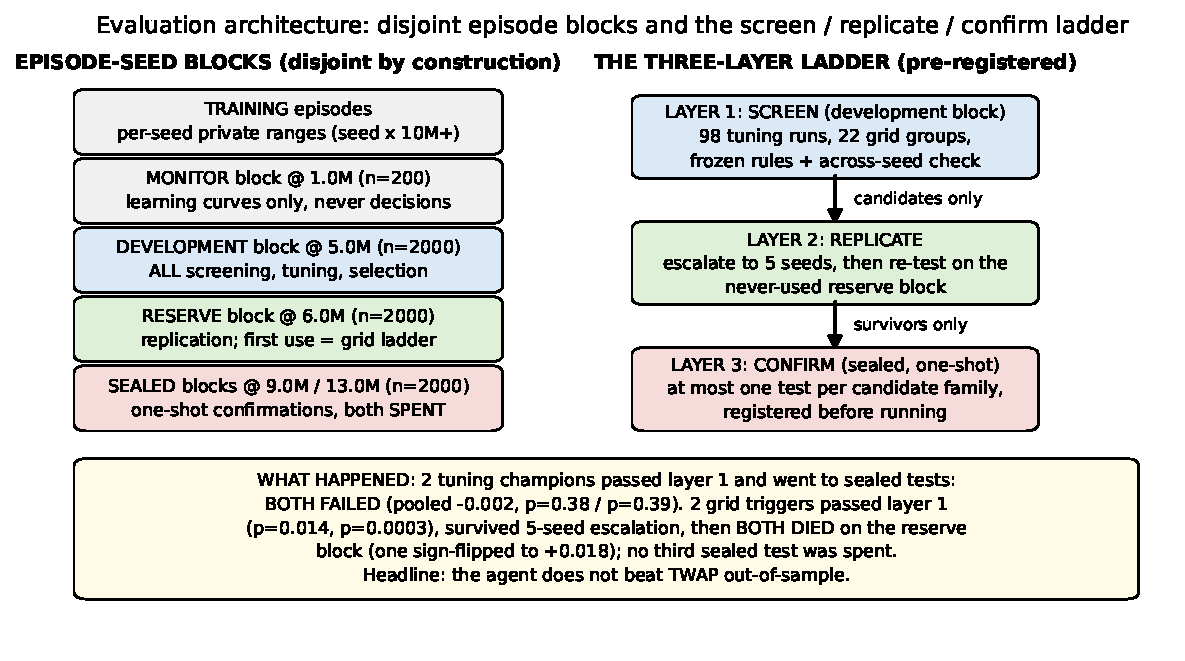
\includegraphics[width=0.9\textwidth]{fig22_pipeline_schematic.pdf}\end{center}
\begin{itemize}
\item Disjoint episode blocks by construction: training ranges (private per seed), a monitor
block (learning curves only), the development block (all screening and selection), a reserve
block (replication), and sealed blocks (one-shot confirmations).
\item Three layers: screen on development data, replicate survivors at five seeds on the
reserve block, confirm once on sealed data.
\item Rationale: roughly 200 configurations were screened on the same development episodes;
under that selection pressure a single validation set is partially used up (winner's curse),
so a replication layer is inserted, as in discovery and replication cohorts.
\item Outcome so far: two champions reached sealed tests and both failed; two grid triggers
died on the reserve block; no sealed test was wasted on them.
\item The replication layer was added mid-project, dated and documented, after the first two
sealed failures; its first use justified it immediately.
\end{itemize}

\subsection*{Environment validation gates (table)}
\begin{center}\resizebox{0.98\textwidth}{!}{% Auto-generated from step4_gates_v3.json + step3g/fairness_verdict_*.json.
\begin{tabular}{llllc}
\toprule
regime & check & measured & pass band & verdict \\
\midrule
calm & own impact is real and persists (2nd immediate dump / 1st, cost ratio) & 2.41 & $\geq 1.25$ & PASS \\
calm & dump cost increases with order size (Spearman $\rho$) & 1.00 & $> 0$ & PASS \\
calm & book refills after impact (probe cost $+30$s vs $+1$s, bps) & -0.46 vs 0.35 & lower at $+30$s & PASS \\
calm & cost-vs-size growth matches the real book (sim vs real ratio) & 2.45 vs 2.46 & within band & PASS \\
calm & fixed-TWAP completes every episode & 100\% & $\geq 99\%$ & PASS \\
calm & dumping costs more than scheduling (dump / TWAP, drift-free, bps) & 0.40 / 0.20 & dump $\geq$ TWAP & PASS \\
calm & no residual background drift (ticks/episode; $t$) & 0.12 ($t$=0.27) & $t$ n.s. & PASS \\
calm & no constant-pace policy beats TWAP (max $|t|$ across paces) & 1.42 & none significant & PASS \\
volatile & own impact is real and persists (2nd immediate dump / 1st, cost ratio) & 2.35 & $\geq 1.25$ & PASS \\
volatile & dump cost increases with order size (Spearman $\rho$) & 1.00 & $> 0$ & PASS \\
volatile & book refills after impact (probe cost $+30$s vs $+1$s, bps) & -0.23 vs 0.14 & lower at $+30$s & PASS \\
volatile & cost-vs-size growth matches the real book (sim vs real ratio) & 2.44 vs 1.99 & within band & PASS \\
volatile & fixed-TWAP completes every episode & 100\% & $\geq 99\%$ & PASS \\
volatile & dumping costs more than scheduling (dump / TWAP, drift-free, bps) & 0.24 / 0.05 & dump $\geq$ TWAP & PASS \\
volatile & no residual background drift (ticks/episode; $t$) & 0.07 ($t$=0.06) & $t$ n.s. & PASS \\
volatile & no constant-pace policy beats TWAP (max $|t|$ across paces) & 1.77 & none significant & PASS \\
\bottomrule
\end{tabular}}\end{center}
\begin{itemize}
\item All gates pass in both regimes, after the drift correction.
\item Self-impact is real and persistent: executing the 25 BTC order makes an identical
immediate follow-on roughly $2.4\times$ more expensive; dump costs are monotone in size.
\item The book demonstrably refills: a probe order is cheaper 30 seconds after the dump than
1 second after.
\item Simulated cost-versus-size growth matches the real books (calm: 2.45 vs 2.46).
\item Fairness gate: residual background drift statistically zero; no constant-pace policy is
significantly cheaper than TWAP (max $|t| = 1.77$), so the benchmark race is fair by
construction.
\end{itemize}

\subsection*{The drift confound, found and fixed}
\begin{center}
\includegraphics[width=0.62\textwidth]{fig6_drift_confound.pdf}\end{center}
\begin{itemize}
\item December 2025 was a rising month; naive replay of its statistics made prices drift
upward in almost every episode, mechanically rewarding fast buying.
\item Caught by an adversarial pre-launch audit before any conclusion was drawn.
\item Fix: drift-neutralised background moves with volatility, spread and impact preserved.
\item The figure shows an identical 20-run design before and after (agents retrained
under each background process): the calm-regime ``edge'' shrinks from $-0.019$\,bps to an
immaterial $-0.006$\,bps, statistically indistinguishable from zero and an order of
magnitude below the $0.05$\,bps materiality floor.
\item A permanent fairness gate now guards this class of bug.
\end{itemize}

\section*{2. Can DRL beat TWAP? The headline}

\subsection*{Primary campaign, all 20 runs (table)}
\begin{center}\resizebox{0.8\textwidth}{!}{% Auto-generated from step5_v3/judgement.json + behaviour_audit.json. Do not edit by hand.
\begin{tabular}{llrrrrc}
\toprule
algo & regime & seed & vs fixed-TWAP & $p_{\mathrm{fix}}$ & vs adaptive-TWAP & valid \\
 & & & (bps) & & (bps) & \\
\midrule
dqn & calm & 0 & +0.1124 & 0.015 & +0.1125 & \textbf{NO} \\
dqn & calm & 1 & +0.0596 & 0.072 & +0.0597 & \textbf{NO} \\
dqn & calm & 2 & +0.0263 & 0.326 & +0.0264 & \textbf{NO} \\
dqn & calm & 3 & +0.1533 & 0.000 & +0.1534 & \textbf{NO} \\
dqn & calm & 4 & -0.0016 & 0.829 & -0.0015 & yes \\
dqn & volatile & 0 & +0.4176 & 0.001 & +0.4169 & \textbf{NO} \\
dqn & volatile & 1 & -0.0296 & 0.632 & -0.0303 & yes \\
dqn & volatile & 2 & +0.3017 & 0.003 & +0.3011 & \textbf{NO} \\
dqn & volatile & 3 & -0.0389 & 0.383 & -0.0396 & yes \\
dqn & volatile & 4 & -0.0197 & 0.893 & -0.0203 & \textbf{NO} \\
ppo & calm & 0 & -0.0108 & 0.958 & -0.0107 & yes \\
ppo & calm & 1 & +0.0110 & 0.576 & +0.0111 & yes \\
ppo & calm & 2 & -0.0194 & 0.324 & -0.0193 & yes \\
ppo & calm & 3 & +0.0020 & 0.597 & +0.0020 & yes \\
ppo & calm & 4 & -0.0108 & 0.632 & -0.0107 & yes \\
ppo & volatile & 0 & -0.0317 & 0.350 & -0.0324 & yes \\
ppo & volatile & 1 & -0.0357 & 0.442 & -0.0364 & yes \\
ppo & volatile & 2 & -0.0892 & 0.012 & -0.0898 & yes \\
ppo & volatile & 3 & -0.0319 & 0.417 & -0.0326 & yes \\
ppo & volatile & 4 & -0.0433 & 0.444 & -0.0439 & yes \\
\bottomrule
\end{tabular}}\end{center}
\begin{itemize}
\item PPO and DQN, calm and volatile, five seeds each, 25 BTC over five minutes, one
decision per second.
\item No cell meets the frozen edge definition. That definition was fixed before any run
and has four parts: the agent must be cheaper than both versions of TWAP; each individual
run must be statistically strong on its own (under one-in-a-hundred odds of chance); the
direction must agree in at least four of the five runs; and the average saving must be at
least 0.05 basis points.
\item All ten PPO runs pass the behaviour audit; seven of ten DQN runs are invalid
(collapse; Section 4).
\item The interesting sub-threshold structure: volatile PPO is cheaper in five of five
seeds.
\item Why that is still not a headline edge: five agreeing directions alone happen by chance
about one time in 32; the average saving (0.047) sits below the 0.05 floor; no single run is
individually significant; and, decisively, the same signal later returned zero on both
sealed tests (Section 2 below).
\end{itemize}

\subsection*{Regime split of the development signal}
\begin{center}
\includegraphics[width=0.6\textwidth]{fig8_regime_comparison.pdf}\end{center}
\begin{itemize}
\item After the drift fix, calm is a tie; the volatile PPO group pools $-0.047$\,bps with
across-seed $p=0.006$.
\item This volatile signal is the candidate edge that everything below chased.
\item Research question 2 note: the signal is regime-specific from the very first campaign.
\end{itemize}

\subsection*{Tuning screen, volatile regime}
\begin{center}
\includegraphics[width=0.66\textwidth]{fig3_forest_tuning_volatile.pdf}\end{center}
\begin{itemize}
\item Twelve pre-registered variants, escalations to five seeds for the leaders.
\item Seven of eight healthy variants reproduce a small consistent advantage: at the time,
strong-looking corroboration; in hindsight, shared evaluation-block luck.
\item Winner: learning rate $10^{-3}$, pooled $-0.063$\,bps, $p=0.0043$ on five seeds.
\item No variant reaches the materiality floor ($-0.05$) with per-seed significance.
\end{itemize}

\subsection*{Tuning screen, calm regime}
\begin{center}
\includegraphics[width=0.66\textwidth]{fig14_forest_tuning_calm.pdf}\end{center}
\begin{itemize}
\item The calm companion: no variant shows a consistent advantage.
\item Confirms the regime asymmetry of the development signal.
\end{itemize}

\subsection*{Tuning and selection summary, all 28 groups (table)}
\begin{center}\resizebox{0.85\textwidth}{!}{% Auto-generated from step5_selection_v3. Do not edit by hand.
\begin{tabular}{lllrrr}
\toprule
variant & change & regime & valid/total & pooled vs adaptive & across-seed \\
 & & & seeds & (bps) & $p$ \\
\midrule
\_v3a & learning rate 1e-3 & volatile & 5/5 & -0.0628 & 0.004 \\
\_v3b & learning rate 1e-4 & volatile & 5/5 & -0.0602 & 0.010 \\
\_v2 & reward x100 & volatile & 5/5 & -0.0462 & 0.002 \\
\_v1b & network 128x128 & volatile & 5/5 & -0.0562 & 0.005 \\
\_v5 & n\_steps 8192 & volatile & 5/5 & -0.0485 & 0.006 \\
\_v4a & ent\_coef 0.0 & volatile & 3/3 & -0.0472 & 0.062 \\
\_v4b & ent\_coef 0.05 & volatile & 5/5 & -0.0267 & 0.048 \\
\_v1a & network 64x64 & volatile & 2/3 & -0.0196 & 0.151 \\
\_v6 & reward x100 @ 10M & volatile & 2/3 & -0.0515 & 0.150 \\
\_v6b & lr 1e-4 @ 10M & volatile & 3/3 & -0.0395 & 0.069 \\
\_w3a & net128 + reward x100 & volatile & 3/3 & -0.0620 & 0.016 \\
\_w3b & lr 1e-4 + reward x100 & volatile & 2/3 & -0.0363 & 0.085 \\
\_d1 & DQN eps 0.05+anneal & volatile & 1/3 & -0.0403 & -- \\
\_d2 & DQN reward x100+net64 & volatile & 3/3 & -0.0259 & 0.199 \\
\midrule
\_v3a & learning rate 1e-3 & calm & 3/3 & +0.0013 & 0.528 \\
\_v3b & learning rate 1e-4 & calm & 2/3 & -0.0239 & 0.111 \\
\_v2 & reward x100 & calm & 3/3 & -0.0024 & 0.322 \\
\_v1b & network 128x128 & calm & 3/3 & -0.0211 & 0.140 \\
\_v5 & n\_steps 8192 & calm & 3/3 & -0.0159 & 0.141 \\
\_v4a & ent\_coef 0.0 & calm & 5/5 & -0.0213 & 0.010 \\
\_v4b & ent\_coef 0.05 & calm & 3/3 & -0.0058 & 0.200 \\
\_v1a & network 64x64 & calm & 3/3 & -0.0159 & 0.040 \\
\_v6 & reward x100 @ 10M & calm & 3/3 & +0.0046 & 0.705 \\
\_v6b & lr 1e-4 @ 10M & calm & 3/3 & -0.0108 & 0.214 \\
\_w3a & net128 + reward x100 & calm & 3/3 & -0.0063 & 0.200 \\
\_w3b & lr 1e-4 + reward x100 & calm & 3/3 & -0.0116 & 0.083 \\
\_d1 & DQN eps 0.05+anneal & calm & 1/3 & -0.0068 & -- \\
\_d2 & DQN reward x100+net64 & calm & 0/3 & -- & -- \\
\bottomrule
\end{tabular}}\end{center}
\begin{itemize}
\item 98 runs in total; every group's pooled result and across-seed consistency.
\item The ten-million-step arms reject the ``it just needed longer training'' explanation.
\item The two DQN remediation variants (d1, d2) do not reliably cure the collapse.
\end{itemize}

\subsection*{Agent configurations (table)}
\begin{center}\resizebox{0.85\textwidth}{!}{% Auto-generated. Base config + each pre-registered variant's single change.
\begin{tabular}{lll}
\toprule
code & agent / variant & change from base \\
\midrule
base (PPO) & PPO, discrete actions & net 30$\times$5, lr 3e-4, reward $\times$1, n\_steps 2048, ent 0.01, 2M steps \\
base (DQN) & DQN, discrete actions & net 30$\times$5, lr 1e-4, buffer 1M, $\varepsilon$ 1.0$\to$0.01 over 25\% \\
\midrule
v1a & bigger network & net\_arch [64, 64] \\
v1b & bigger network & net\_arch [128, 128] \\
v2 & stronger feedback & reward scale $\times$100 \\
v3a & faster learning & learning rate 1e-3 \\
v3b & slower learning & learning rate 1e-4 \\
v4a & no exploration bonus & ent\_coef 0.0 \\
v4b & more exploration & ent\_coef 0.05 \\
v5 & longer rollout & n\_steps 8192 \\
v6 & v2 trained longer & reward $\times$100, 10M steps \\
v6b & v3b trained longer & lr 1e-4, 10M steps \\
w3a & combination & net [128,128] + reward $\times$100 \\
w3b & combination & lr 1e-4 + reward $\times$100 \\
d1 & DQN collapse fix & exploration\_final\_eps 0.05, anneal 0.5 \\
d2 & DQN collapse fix & reward $\times$100 + net [64,64] \\
\bottomrule
\end{tabular}}\end{center}
\begin{itemize}
\item Base PPO and DQN share the same $30\times5$ network, discount factor and observation
set, and matched gradient sample throughput (${\sim}20$M sample-passes per run): the
algorithm comparison is compute-fair.
\item Each variant changes exactly one named thing (two for the combination arms).
\end{itemize}

\clearpage
\subsection*{Full tuning campaign, all 98 runs (appendix table)}
\begin{itemize}
\item The complete run-level record behind the group summary: every seed, both benchmarks,
audit outcome. The table flows over the following pages.
\item Included so no result is summarised away; the source files are listed in the
provenance table at the end.
\end{itemize}
\begin{center}\scriptsize% Auto-generated from step5_selection_v3 (all 98 tuning-campaign runs, per seed).
% LONGTABLE: flows across pages; include directly (no float, no resizebox).
\begin{longtable}{lllrrrrc}
\toprule
algo & regime & variant & seed & vs fixed & $p$ & vs adaptive & valid \\
\midrule
\endhead
dqn & calm & \_d1 & 0 & +0.0894 & 0.002 & +0.0895 & \textbf{NO} \\
dqn & calm & \_d1 & 1 & -0.0069 & 0.780 & -0.0068 & yes \\
dqn & calm & \_d1 & 2 & -0.0068 & 0.838 & -0.0067 & \textbf{NO} \\
dqn & calm & \_d2 & 0 & +0.1442 & 0.002 & +0.1443 & \textbf{NO} \\
dqn & calm & \_d2 & 1 & +0.1393 & 0.001 & +0.1393 & \textbf{NO} \\
dqn & calm & \_d2 & 2 & +0.0099 & 0.604 & +0.0100 & \textbf{NO} \\
dqn & volatile & \_d1 & 0 & +0.1398 & 0.157 & +0.1392 & \textbf{NO} \\
dqn & volatile & \_d1 & 1 & +0.0324 & 0.307 & +0.0318 & \textbf{NO} \\
dqn & volatile & \_d1 & 2 & -0.0396 & 0.334 & -0.0403 & yes \\
dqn & volatile & \_d2 & 0 & +0.0063 & 0.675 & +0.0057 & yes \\
dqn & volatile & \_d2 & 1 & -0.0729 & 0.032 & -0.0736 & yes \\
dqn & volatile & \_d2 & 2 & -0.0092 & 0.709 & -0.0099 & yes \\
ppo & calm & \_v1a & 0 & -0.0226 & 0.248 & -0.0225 & yes \\
ppo & calm & \_v1a & 1 & -0.0068 & 0.770 & -0.0067 & yes \\
ppo & calm & \_v1a & 2 & -0.0185 & 0.243 & -0.0184 & yes \\
ppo & calm & \_v1b & 0 & +0.0053 & 0.960 & +0.0054 & yes \\
ppo & calm & \_v1b & 1 & -0.0246 & 0.196 & -0.0245 & yes \\
ppo & calm & \_v1b & 2 & -0.0441 & 0.016 & -0.0441 & yes \\
ppo & calm & \_v2 & 0 & -0.0111 & 0.732 & -0.0110 & yes \\
ppo & calm & \_v2 & 1 & +0.0001 & 0.787 & +0.0002 & yes \\
ppo & calm & \_v2 & 2 & +0.0036 & 0.958 & +0.0036 & yes \\
ppo & calm & \_v3a & 0 & +0.0337 & 0.070 & +0.0338 & yes \\
ppo & calm & \_v3a & 1 & -0.0230 & 0.230 & -0.0229 & yes \\
ppo & calm & \_v3a & 2 & -0.0069 & 0.607 & -0.0068 & yes \\
ppo & calm & \_v3b & 0 & -0.0327 & 0.089 & -0.0326 & yes \\
ppo & calm & \_v3b & 1 & -0.0153 & 0.623 & -0.0153 & yes \\
ppo & calm & \_v3b & 2 & -0.0148 & 0.426 & -0.0147 & \textbf{NO} \\
ppo & calm & \_v4a & 0 & -0.0189 & 0.416 & -0.0188 & yes \\
ppo & calm & \_v4a & 1 & -0.0126 & 0.515 & -0.0125 & yes \\
ppo & calm & \_v4a & 2 & -0.0298 & 0.370 & -0.0298 & yes \\
ppo & calm & \_v4a & 3 & -0.0382 & 0.028 & -0.0381 & yes \\
ppo & calm & \_v4a & 4 & -0.0076 & 0.872 & -0.0075 & yes \\
ppo & calm & \_v4b & 0 & +0.0027 & 0.986 & +0.0028 & yes \\
ppo & calm & \_v4b & 1 & -0.0161 & 0.444 & -0.0161 & yes \\
ppo & calm & \_v4b & 2 & -0.0043 & 0.808 & -0.0042 & yes \\
ppo & calm & \_v5 & 0 & -0.0068 & 0.808 & -0.0067 & yes \\
ppo & calm & \_v5 & 1 & -0.0035 & 0.915 & -0.0034 & yes \\
ppo & calm & \_v5 & 2 & -0.0377 & 0.047 & -0.0376 & yes \\
ppo & calm & \_v6 & 0 & +0.0135 & 0.671 & +0.0136 & yes \\
ppo & calm & \_v6 & 1 & +0.0100 & 0.996 & +0.0100 & yes \\
ppo & calm & \_v6 & 2 & -0.0099 & 0.872 & -0.0098 & yes \\
ppo & calm & \_v6b & 0 & -0.0319 & 0.066 & -0.0318 & yes \\
ppo & calm & \_v6b & 1 & +0.0047 & 0.687 & +0.0047 & yes \\
ppo & calm & \_v6b & 2 & -0.0053 & 0.573 & -0.0052 & yes \\
ppo & calm & \_w3a & 0 & +0.0017 & 0.901 & +0.0018 & yes \\
ppo & calm & \_w3a & 1 & -0.0178 & 0.287 & -0.0177 & yes \\
ppo & calm & \_w3a & 2 & -0.0029 & 0.841 & -0.0029 & yes \\
ppo & calm & \_w3b & 0 & -0.0218 & 0.235 & -0.0217 & yes \\
ppo & calm & \_w3b & 1 & -0.0102 & 0.785 & -0.0101 & yes \\
ppo & calm & \_w3b & 2 & -0.0032 & 0.648 & -0.0031 & yes \\
ppo & volatile & \_v1a & 0 & -0.0089 & 0.803 & -0.0096 & yes \\
ppo & volatile & \_v1a & 1 & -0.0290 & 0.374 & -0.0296 & yes \\
ppo & volatile & \_v1a & 2 & +0.0232 & 0.546 & +0.0226 & \textbf{NO} \\
ppo & volatile & \_v1b & 0 & -0.0150 & 0.573 & -0.0156 & yes \\
ppo & volatile & \_v1b & 1 & -0.0436 & 0.196 & -0.0443 & yes \\
ppo & volatile & \_v1b & 2 & -0.0640 & 0.071 & -0.0646 & yes \\
ppo & volatile & \_v1b & 3 & -0.0870 & 0.020 & -0.0876 & yes \\
ppo & volatile & \_v1b & 4 & -0.0684 & 0.051 & -0.0691 & yes \\
ppo & volatile & \_v2 & 0 & -0.0501 & 0.168 & -0.0507 & yes \\
ppo & volatile & \_v2 & 1 & -0.0615 & 0.119 & -0.0621 & yes \\
ppo & volatile & \_v2 & 2 & -0.0519 & 0.186 & -0.0525 & yes \\
ppo & volatile & \_v2 & 3 & -0.0495 & 0.156 & -0.0502 & yes \\
ppo & volatile & \_v2 & 4 & -0.0150 & 0.965 & -0.0156 & yes \\
ppo & volatile & \_v3a & 0 & -0.0494 & 0.243 & -0.0500 & yes \\
ppo & volatile & \_v3a & 1 & -0.1044 & 0.012 & -0.1050 & yes \\
ppo & volatile & \_v3a & 2 & -0.0345 & 0.369 & -0.0352 & yes \\
ppo & volatile & \_v3a & 3 & -0.0798 & 0.023 & -0.0805 & yes \\
ppo & volatile & \_v3a & 4 & -0.0427 & 0.236 & -0.0433 & yes \\
ppo & volatile & \_v3b & 0 & -0.0717 & 0.047 & -0.0724 & yes \\
ppo & volatile & \_v3b & 1 & -0.1019 & 0.006 & -0.1026 & yes \\
ppo & volatile & \_v3b & 2 & -0.0759 & 0.038 & -0.0765 & yes \\
ppo & volatile & \_v3b & 3 & -0.0089 & 0.866 & -0.0095 & yes \\
ppo & volatile & \_v3b & 4 & -0.0394 & 0.344 & -0.0401 & yes \\
ppo & volatile & \_v4a & 0 & -0.0501 & 0.188 & -0.0508 & yes \\
ppo & volatile & \_v4a & 1 & -0.0764 & 0.018 & -0.0771 & yes \\
ppo & volatile & \_v4a & 2 & -0.0131 & 0.944 & -0.0137 & yes \\
ppo & volatile & \_v4b & 0 & -0.0402 & 0.266 & -0.0408 & yes \\
ppo & volatile & \_v4b & 1 & -0.0380 & 0.334 & -0.0387 & yes \\
ppo & volatile & \_v4b & 2 & -0.0231 & 0.422 & -0.0238 & yes \\
ppo & volatile & \_v4b & 3 & -0.0492 & 0.154 & -0.0498 & yes \\
ppo & volatile & \_v4b & 4 & +0.0201 & 0.682 & +0.0195 & yes \\
ppo & volatile & \_v5 & 0 & -0.0506 & 0.156 & -0.0512 & yes \\
ppo & volatile & \_v5 & 1 & -0.0211 & 0.698 & -0.0217 & yes \\
ppo & volatile & \_v5 & 2 & -0.0261 & 0.454 & -0.0267 & yes \\
ppo & volatile & \_v5 & 3 & -0.0779 & 0.056 & -0.0785 & yes \\
ppo & volatile & \_v5 & 4 & -0.0637 & 0.124 & -0.0643 & yes \\
ppo & volatile & \_v6 & 0 & -0.0245 & 0.829 & -0.0252 & yes \\
ppo & volatile & \_v6 & 1 & -0.0772 & 0.083 & -0.0778 & yes \\
ppo & volatile & \_v6 & 2 & -0.0295 & 0.608 & -0.0302 & \textbf{NO} \\
ppo & volatile & \_v6b & 0 & -0.0620 & 0.093 & -0.0627 & yes \\
ppo & volatile & \_v6b & 1 & -0.0073 & 0.976 & -0.0079 & yes \\
ppo & volatile & \_v6b & 2 & -0.0474 & 0.151 & -0.0480 & yes \\
ppo & volatile & \_w3a & 0 & -0.0602 & 0.100 & -0.0609 & yes \\
ppo & volatile & \_w3a & 1 & -0.0814 & 0.029 & -0.0821 & yes \\
ppo & volatile & \_w3a & 2 & -0.0423 & 0.470 & -0.0430 & yes \\
ppo & volatile & \_w3b & 0 & -0.0456 & 0.153 & -0.0462 & yes \\
ppo & volatile & \_w3b & 1 & +0.0471 & 0.467 & +0.0465 & \textbf{NO} \\
ppo & volatile & \_w3b & 2 & -0.0257 & 0.647 & -0.0263 & yes \\
\bottomrule
\end{longtable}\end{center}
\clearpage

\subsection*{Training curves}
\begin{center}
\includegraphics[width=0.6\textwidth]{fig5_learning_curves_volatile.pdf}\end{center}
\begin{itemize}
\item Base and selected configurations plateau; training ran to completion at 2M steps.
\item Measured on the monitor block, which is never used for decisions.
\item No sign that the null is under-training in disguise.
\end{itemize}

\subsection*{Both sealed confirmations (table)}
\begin{center}\resizebox{0.85\textwidth}{!}{% Auto-generated from step5_confirm_v3a (9e6) + step5_confirm_v1b (13e6).
\begin{tabular}{lllrrrc}
\toprule
config & sealed block & seed & vs fixed & vs adaptive & $p$ (adaptive) & valid \\
\midrule
faster-learning (v3a) & 9{,}000{,}000 & 5 & +0.0221 & +0.0222 & 0.749 & yes \\
 &  & 6 & -0.0104 & -0.0103 & 0.813 & yes \\
 &  & 7 & +0.0028 & +0.0028 & 0.804 & yes \\
 &  & 8 & -0.0080 & -0.0079 & 0.936 & yes \\
 &  & 9 & -0.0184 & -0.0184 & 0.758 & yes \\
\cmidrule(lr){2-7}
 & \multicolumn{6}{l}{pooled vs adaptive = -0.0023 bps; across-seed $p$ = 0.379; cheaper in 3/5; \textbf{PASS = FALSE}} \\
\midrule
bigger-network (v1b) & 13{,}000{,}000 & 10 & -0.0010 & -0.0019 & 0.650 & yes \\
 &  & 11 & +0.0042 & +0.0033 & 0.953 & yes \\
 &  & 12 & -0.0297 & -0.0306 & 0.294 & yes \\
 &  & 13 & +0.0153 & +0.0144 & 0.491 & yes \\
 &  & 14 & +0.0047 & +0.0038 & 0.961 & yes \\
\cmidrule(lr){2-7}
 & \multicolumn{6}{l}{pooled vs adaptive = -0.0022 bps; across-seed $p$ = 0.394; cheaper in 2/5; \textbf{PASS = FALSE}} \\
\bottomrule
\end{tabular}}\end{center}
\begin{itemize}
\item Two champions (one chosen on volatile-regime performance, one chosen by the
pre-registered selection rule applied exactly as written), five fresh seeds each, evaluated
once on separate never-used sealed blocks.
\item Results: $-0.0023$\,bps ($p=0.379$, 3/5 cheaper) and $-0.0022$\,bps ($p=0.394$, 2/5
cheaper); both confidence intervals bracket zero.
\item Testing the second candidate also resolved a disclosed selection-metric ambiguity
empirically: both picks are approximately zero out of sample.
\item The confirmation family was capped at two tests in advance; no re-runs.
\end{itemize}

\subsection*{The headline figure}
\begin{center}
\includegraphics[width=0.62\textwidth]{fig1_dev_vs_sealed.pdf}\end{center}
\begin{itemize}
\item Development-block advantage versus sealed reality, both champions side by side.
\item The signal that was consistent across five seeds and twelve variants does not exist on
fresh data.
\item Headline of the dissertation: a boundary null, established twice under pre-committed
rules.
\end{itemize}

\subsection*{Why the illusion is visible in hindsight}
\begin{center}
\includegraphics[width=0.62\textwidth]{fig4_three_block_signflip.pdf}\end{center}
\begin{itemize}
\item The same configurations on three disjoint blocks: worse than TWAP on the monitor
block, better on the development block, zero on sealed blocks.
\item Seed agreement cannot detect shared evaluation-set luck: every seed is graded on the
same episodes.
\item This is demonstration number two of the spurious-edge anatomy (the drift was number
one; the grid triggers below are number three).
\end{itemize}

\subsection*{Absolute cost distributions}
\begin{center}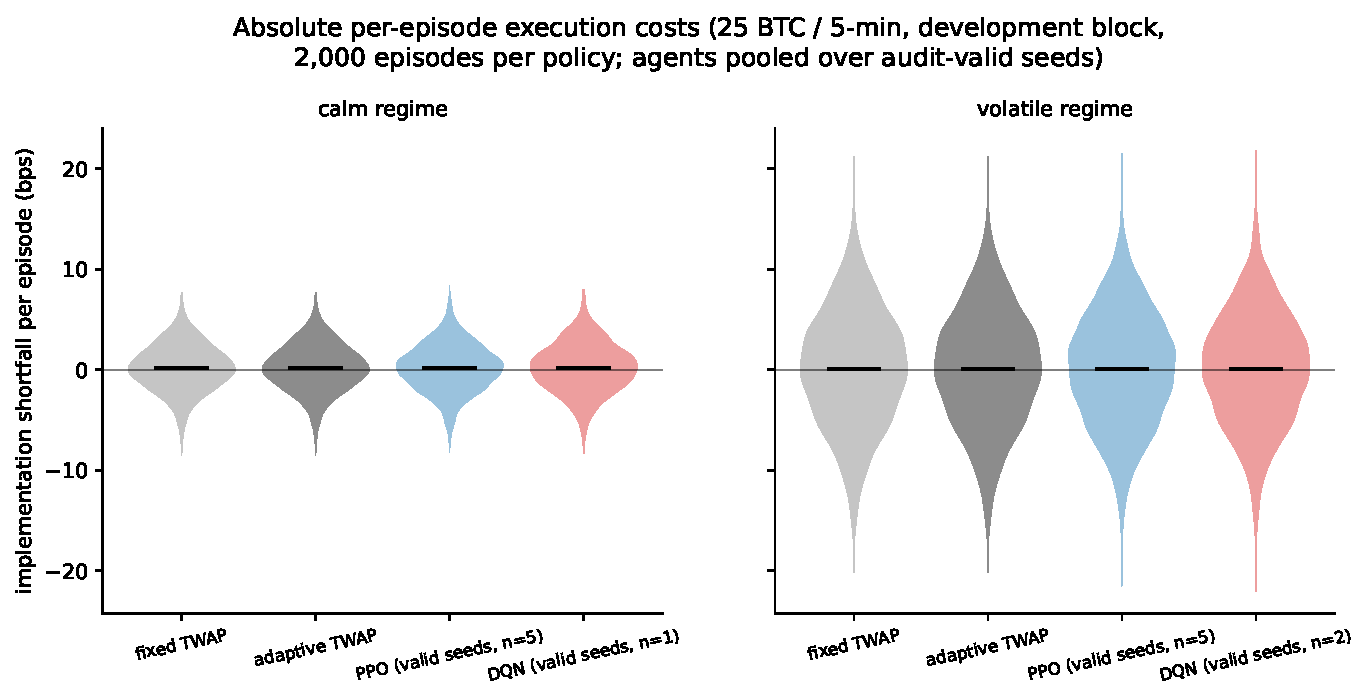
\includegraphics[width=0.9\textwidth]{fig10a_cost_distributions.pdf}\end{center}
\begin{itemize}
\item What each shape is: one violin summarises the 2{,}000 individual episode costs of one
policy; the wider the shape at a given height, the more episodes cost that amount.
\item How to read the axis: the vertical axis is the cost of executing the 25 BTC order in
basis points relative to the price at the start of the episode; positive means the policy
paid more than the arrival price, negative means it paid less.
\item The black bar inside each violin is that policy's average cost; all four averages sit
essentially at zero in both panels.
\item The key comparison: within each panel the four shapes (fixed TWAP, adaptive TWAP,
PPO, DQN) are nearly identical, so the choice of policy barely changes what execution
costs; the market decides, not the policy.
\item Regime effect: the volatile panel's shapes span roughly $-20$ to $+20$ basis points
versus roughly $-8$ to $+8$ in calm, so volatility widens the cost distribution by about a
factor of 2.5 for every policy equally (sd 2.35 to 5.88 bps).
\item Trust in the data: this replay provably describes the same evaluations as the sealed
verdicts, because every recomputed average matches the sealed record exactly (20 of 20
runs).
\end{itemize}

\subsection*{Paired per-episode differences}
\begin{center}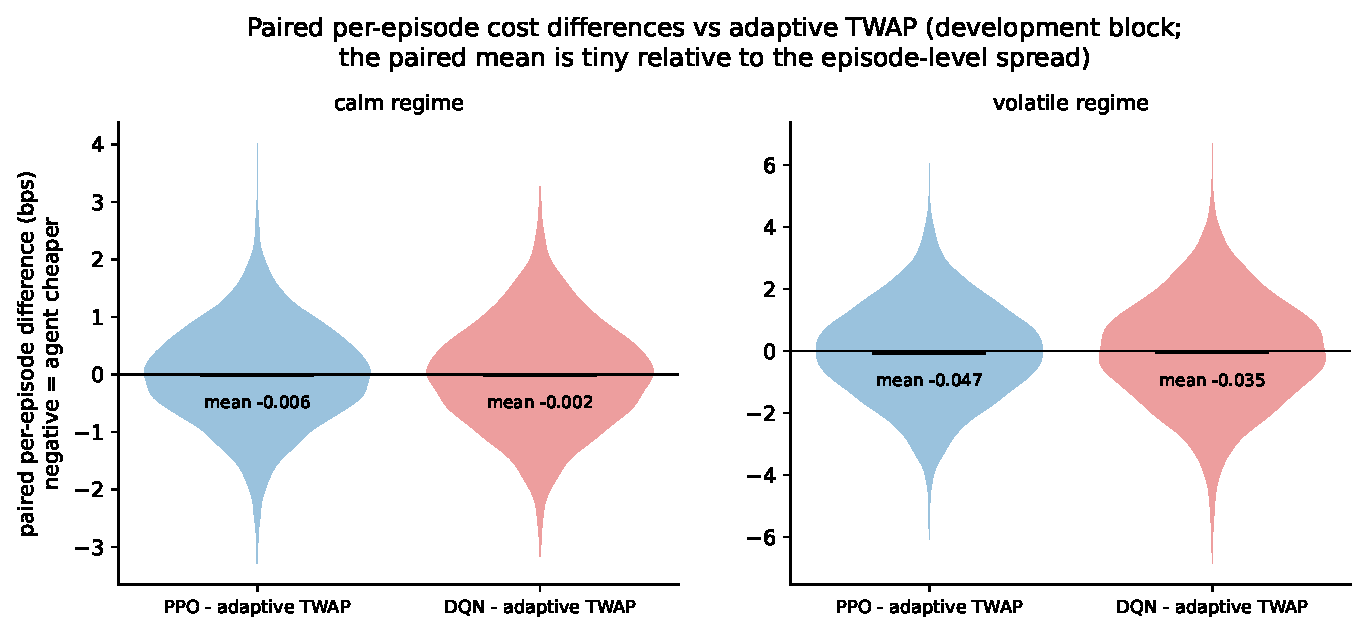
\includegraphics[width=0.9\textwidth]{fig10b_paired_distributions.pdf}\end{center}
\begin{itemize}
\item The paired agent-minus-benchmark differences, pooled over audit-valid seeds.
\item The paired mean ($-0.047$ at best) is three orders of magnitude smaller than the
episode-level spread.
\item This is the visual justification for 2{,}000 paired episodes and strict statistical
discipline: anything less and noise decides.
\end{itemize}

\subsection*{Descriptive statistics (table)}
\begin{center}\resizebox{0.9\textwidth}{!}{% Auto-generated from per_episode_v3/*.npz (deterministic replay; integrity
% exact vs step5_v3/judgement.json for all 20 runs).
\begin{tabular}{llrrrrrr}
\toprule
regime & policy & mean & sd & median & 5\% & 95\% & $n$ episodes \\
\midrule
calm & fixed TWAP & +0.1803 & 2.3546 & +0.1840 & -3.7238 & +4.0427 & 2{,}000 \\
calm & adaptive TWAP & +0.1802 & 2.3540 & +0.1810 & -3.7212 & +4.0245 & 2{,}000 \\
calm & PPO (valid seeds) & +0.1747 & 2.3661 & +0.2089 & -3.7477 & +3.9982 & 10{,}000 \\
calm & DQN (valid seeds) & +0.1787 & 2.4817 & +0.1849 & -3.9363 & +4.2143 & 2{,}000 \\
\midrule
volatile & fixed TWAP & +0.1031 & 5.8800 & +0.1013 & -9.7930 & +9.4489 & 2{,}000 \\
volatile & adaptive TWAP & +0.1037 & 5.8793 & +0.0922 & -9.7133 & +9.4541 & 2{,}000 \\
volatile & PPO (valid seeds) & +0.0567 & 5.7882 & +0.1640 & -9.3214 & +9.2684 & 10{,}000 \\
volatile & DQN (valid seeds) & +0.0688 & 5.6446 & +0.1161 & -9.0810 & +9.1627 & 4{,}000 \\
\bottomrule
\end{tabular}}\end{center}
\begin{itemize}
\item Mean, spread, median and 5/95 percentiles per policy and regime.
\item Medians sit near zero everywhere; tails are wide and symmetric; no policy shifts the
distribution visibly.
\end{itemize}

\section*{3. Robustness: the null holds everywhere}

\subsection*{Size response}
\begin{center}
\includegraphics[width=0.58\textwidth]{fig2_size_response.pdf}\end{center}
\begin{itemize}
\item A genuine impact-management edge should grow with order size.
\item Instead the signal exists only at the 25 BTC development size and is absent at 5,
12.5 and 50 BTC: non-monotone, the signature of selection on noise.
\item This was the fourth independent line of evidence against the development edge, before
the grid.
\end{itemize}

\subsection*{The full grid}
\begin{center}
\includegraphics[width=0.92\textwidth]{fig9_grid_heatmap.pdf}\end{center}
\begin{itemize}
\item 66 new runs completing sizes $\{5,12.5,25,50\}$ BTC by deadlines $\{2.5,5,10,20\}$
minutes, both regimes; integrity-checked before judging.
\item Null in 20 of 22 new groups; several groups significantly worse than TWAP (e.g.
12.5 BTC at 20 minutes, volatile: $+0.164$\,bps).
\item Two calm cells (solid outline) met the pre-registered follow-up trigger; the centre
volatile cell (dashed) is the already-falsified original signal.
\end{itemize}

\subsection*{Grid summary (table)}
\begin{center}\resizebox{0.8\textwidth}{!}{% Auto-generated from step5_grid_* + step5_sweep_* + step5_selection_v3. Do not edit.
\begin{tabular}{llrrrrrc}
\toprule
regime & deadline & size & valid/ & cheaper & pooled vs & across-seed & follow-up \\
 & (min) & (BTC) & total & & adaptive (bps) & $p$ & trigger \\
\midrule
calm & 2.5 & 5 & 3/3 & 2/3 & -0.0094 & 0.2498 & no \\
 & 2.5 & 12.5 & 3/3 & 1/3 & +0.0032 & 0.7761 & no \\
 & 2.5 & 25 & 2/3 & 1/2 & +0.0029 & 0.5919 & no \\
 & 2.5 & 50 & 2/3 & 0/2 & +0.0060 & 0.9525 & no \\
 & 5 & 5 & 3/3 & 2/3 & -0.0142 & 0.1346 & no \\
 & 5 & 12.5 & 3/3 & 2/3 & -0.0233 & 0.1191 & no \\
 & 5 & 25 & 3/3 & 2/3 & +0.0013 & 0.5279 & no \\
 & 5 & 50 & 3/3 & 0/3 & +0.0100 & 0.9757 & no \\
 & 10 & 5 & 3/3 & 1/3 & +0.0105 & 0.8819 & no \\
 & 10 & 12.5 & 3/3 & 3/3 & -0.0178 & 0.0261 & no \\
 & 10 & 25 & 3/3 & 3/3 & -0.0250 & 0.0646 & no \\
 & 10 & 50 & 3/3 & 3/3 & -0.0539 & 0.0140 & \textbf{YES} \\
 & 20 & 5 & 3/3 & 0/3 & +0.0338 & 0.9991 & no \\
 & 20 & 12.5 & 3/3 & 1/3 & +0.0189 & 0.8863 & no \\
 & 20 & 25 & 3/3 & 3/3 & -0.0629 & 0.0003 & \textbf{YES} \\
 & 20 & 50 & 3/3 & 2/3 & -0.0169 & 0.3466 & no \\
\midrule
volatile & 2.5 & 5 & 3/3 & 2/3 & -0.0132 & 0.1492 & no \\
 & 2.5 & 12.5 & 3/3 & 1/3 & +0.0126 & 0.7186 & no \\
 & 2.5 & 25 & 3/3 & 3/3 & -0.0134 & 0.0273 & no \\
 & 2.5 & 50 & 3/3 & 0/3 & +0.0301 & 0.9740 & no \\
 & 5 & 5 & 3/3 & 0/3 & +0.0426 & 0.9526 & no \\
 & 5 & 12.5 & 2/3 & 2/2 & -0.0159 & 0.1424 & no \\
 & 5 & 25 & 5/5 & 5/5 & -0.0628 & 0.0043 & closed (failed both sealed tests) \\
 & 5 & 50 & 3/3 & 1/3 & +0.0024 & 0.6120 & no \\
 & 10 & 5 & 3/3 & 2/3 & -0.0383 & 0.1503 & no \\
 & 10 & 12.5 & 3/3 & 3/3 & -0.0262 & 0.1180 & no \\
 & 10 & 25 & 3/3 & 2/3 & -0.0619 & 0.1123 & no \\
 & 10 & 50 & 3/3 & 3/3 & -0.0821 & 0.0833 & no \\
 & 20 & 5 & 3/3 & 0/3 & +0.0648 & 0.8996 & no \\
 & 20 & 12.5 & 3/3 & 0/3 & +0.1638 & 0.9926 & no \\
 & 20 & 25 & 3/3 & 2/3 & +0.0156 & 0.6764 & no \\
 & 20 & 50 & 3/3 & 1/3 & +0.0150 & 0.6099 & no \\
\bottomrule
\end{tabular}}\end{center}
\begin{itemize}
\item All 16 cells per regime with pooled results, consistency, and trigger status.
\item Roughly one false trigger was expected among 22 groups by chance; two were observed,
hence follow-up rather than claims.
\end{itemize}

\subsection*{The replication ladder kills both triggers}
\begin{center}
\includegraphics[width=0.62\textwidth]{fig19_ladder_collapse.pdf}\end{center}
\begin{itemize}
\item The triggers: $p=0.014$, and $p=0.0003$ with three seeds within $0.005$\,bps of one
another.
\item Both survived escalation to five seeds on the development block ($p=0.0037$ and
$p=0.0001$).
\item Both then died on the first-ever use of the reserve block: $-0.0095$ ($p=0.17$) and
$+0.0177$ ($p=0.96$), the second reversing sign entirely.
\item Cost of catching it: four training runs. Sealed tests spent: zero.
\item Third demonstrated evaluation-set illusion, and the cleanest.
\end{itemize}

\subsection*{Ladder detail (table)}
\begin{center}% Auto-generated from step5_esc_* (development block, 5 seeds) and step5_xblock_*
% (reserve block, first use). The two grid trigger groups, calm regime.
\begin{tabular}{llrrr}
\toprule
group & seed & development (bps) & reserve (bps) & change \\
\midrule
50 BTC / 10-min & 0 & -0.0453 & -0.0028 & +0.0425 \\
 & 1 & -0.0723 & +0.0122 & +0.0846 \\
 & 2 & -0.0441 & -0.0418 & +0.0023 \\
 & 3 & -0.0346 & -0.0056 & +0.0290 \\
 & 4 & -0.0196 & -0.0097 & +0.0099 \\
 & pooled & -0.0432 & -0.0095 & +0.0336 \\
\midrule
25 BTC / 20-min & 0 & -0.0601 & +0.0120 & +0.0721 \\
 & 1 & -0.0640 & +0.0397 & +0.1037 \\
 & 2 & -0.0647 & -0.0058 & +0.0589 \\
 & 3 & -0.0721 & +0.0244 & +0.0964 \\
 & 4 & -0.0435 & +0.0182 & +0.0617 \\
 & pooled & -0.0609 & +0.0177 & +0.0786 \\
\bottomrule
\end{tabular}\end{center}
\begin{itemize}
\item Every escalated seed's development and reserve result side by side.
\item Note the tight development agreement dissolving into scatter around zero on fresh
episodes.
\end{itemize}

\section*{4. Why DQN fails}

\subsection*{The collapse at the primary setting}
\begin{center}
\includegraphics[width=0.9\textwidth]{fig7_dqn_collapse.pdf}\end{center}
\begin{itemize}
\item The behaviour audit runs before any cost comparison: an agent whose forced deadline
purchase completes more than $10\%$ of episodes, or that is more than $90\%$ inactive, is
invalid.
\item Seven of ten DQN agents collapse into inaction followed by the forced purchase; all
ten PPO agents trade properly.
\item Collapsed agents' cost numbers are excluded from verdicts but always reported.
\end{itemize}

\subsection*{Systematic, size-driven, and not a configuration artifact}
\begin{center}
\includegraphics[width=0.66\textwidth]{fig20_dqn_collapse_by_setting.pdf}\end{center}
\begin{itemize}
\item Pre-registered probe across settings: mostly healthy at 5 BTC (4/6 valid), total
collapse at 25 BTC even at the shortest deadline (0/6), majority collapse at every 25 BTC
deadline.
\item So the driver is order size (reward dominated by the agent's own impact), not idle
time; the going-in idle-room hypothesis was refuted by the probe's own design.
\item The collapse concentrates in the calm regime (1 of 9 calm probe agents valid versus
5 of 9 volatile).
\item Grey bars: retraining with the library-default update rhythm (18 runs, pre-registered)
leaves the primary setting unchanged; the rhythm objection is closed with data.
\end{itemize}

\subsection*{DQN probe detail (table)}
\begin{center}\resizebox{0.85\textwidth}{!}{% Auto-generated from step5_dqnprobe_* (criteria Part D, 18 runs).
\begin{tabular}{llrrrrrc}
\toprule
cell & regime & seed & do-nothing & forced-buy & vs adaptive & $p$ & audit \\
 & & & share & share & (bps) & & \\
\midrule
5 BTC / 2.5-min & calm & 0 & 93\% & 43\% & -0.0287 & 0.425 & \textbf{COLL.} \\
5 BTC / 2.5-min & calm & 1 & 36\% & 22\% & -0.0250 & 0.159 & \textbf{COLL.} \\
5 BTC / 2.5-min & calm & 2 & 6\% & 2\% & +0.0036 & 0.824 & valid \\
5 BTC / 2.5-min & volatile & 0 & 7\% & 0\% & +0.0316 & 0.309 & valid \\
5 BTC / 2.5-min & volatile & 1 & 43\% & 0\% & -0.0540 & 0.176 & valid \\
5 BTC / 2.5-min & volatile & 2 & 1\% & 0\% & -0.0406 & 0.041 & valid \\
\midrule
25 BTC / 2.5-min & calm & 0 & 82\% & 100\% & +0.0258 & 0.500 & \textbf{COLL.} \\
25 BTC / 2.5-min & calm & 1 & 57\% & 18\% & -0.0089 & 0.646 & \textbf{COLL.} \\
25 BTC / 2.5-min & calm & 2 & 13\% & 67\% & -0.0223 & 0.179 & \textbf{COLL.} \\
25 BTC / 2.5-min & volatile & 0 & 17\% & 48\% & -0.0410 & 0.529 & \textbf{COLL.} \\
25 BTC / 2.5-min & volatile & 1 & 46\% & 12\% & -0.0523 & 0.247 & \textbf{COLL.} \\
25 BTC / 2.5-min & volatile & 2 & 37\% & 72\% & -0.0106 & 0.828 & \textbf{COLL.} \\
\midrule
25 BTC / 20-min & calm & 0 & 43\% & 54\% & -0.0518 & 0.088 & \textbf{COLL.} \\
25 BTC / 20-min & calm & 1 & 43\% & 87\% & -0.0019 & 0.866 & \textbf{COLL.} \\
25 BTC / 20-min & calm & 2 & 54\% & 70\% & -0.0462 & 0.346 & \textbf{COLL.} \\
25 BTC / 20-min & volatile & 0 & 16\% & 8\% & -0.2288 & 0.025 & valid \\
25 BTC / 20-min & volatile & 1 & 30\% & 0\% & -0.0539 & 0.427 & valid \\
25 BTC / 20-min & volatile & 2 & 25\% & 78\% & -0.0193 & 0.570 & \textbf{COLL.} \\
\bottomrule
\end{tabular}}\end{center}
\begin{itemize}
\item All 18 probe runs: inaction share, forced-purchase share, costs, audit outcome.
\item Even where DQN survives the audit, no cost advantage exists anywhere.
\end{itemize}

\subsection*{The mechanism, read from the networks}
\begin{center}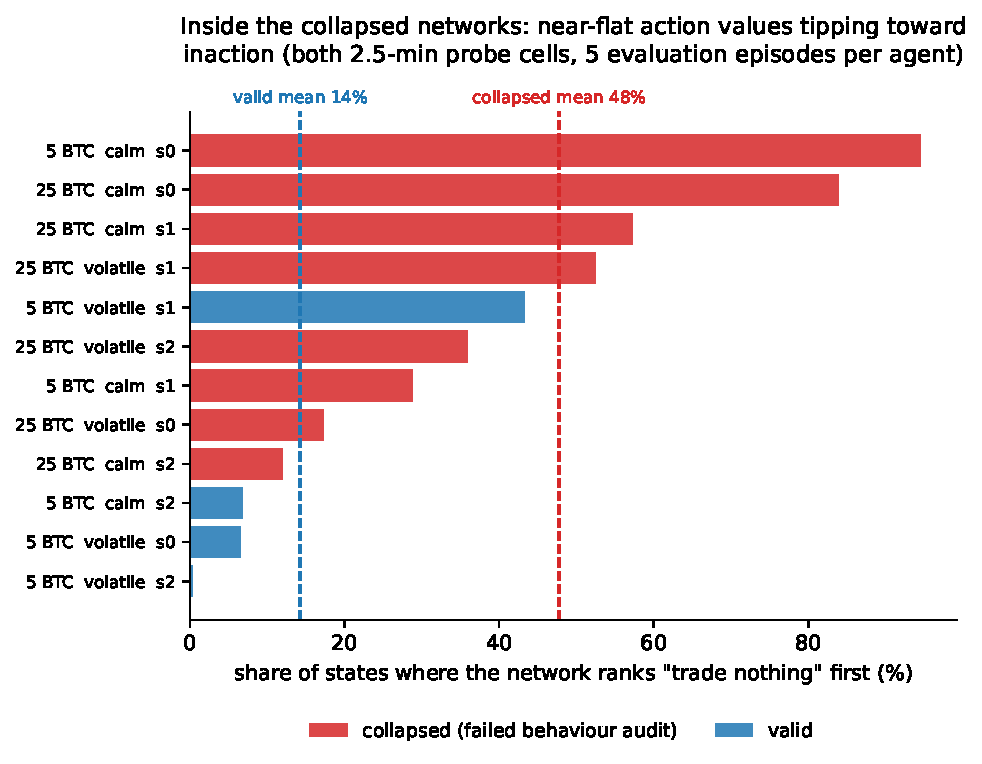
\includegraphics[width=0.66\textwidth]{fig21_q_tilt.pdf}\end{center}
\begin{itemize}
\item Direct inspection of the trained networks over evaluation states.
\item Across all agents, learned action-value separations ($0.006$ to $0.012$) sit an order
of magnitude below per-step reward noise (sd $0.025$ to $0.057$): the value signal is at
the edge of resolvability for everyone.
\item What distinguishes collapse is where the near-flat surface tips: collapsed agents rank
``trade nothing'' first in $48\%$ of states versus $14\%$ for healthy agents.
\item Interpretation (labelled as such): PPO's batch-normalised advantages amplify
microscopic differences; DQN regresses raw-scale values.
\item Scoped claim: this configuration on impact-dominated rewards; Double-DQN and
prioritised replay are named future work.
\end{itemize}

\section*{5. The frozen-replay track (validation results; sealed exam pending)}

\subsection*{Three-lever null}
\begin{center}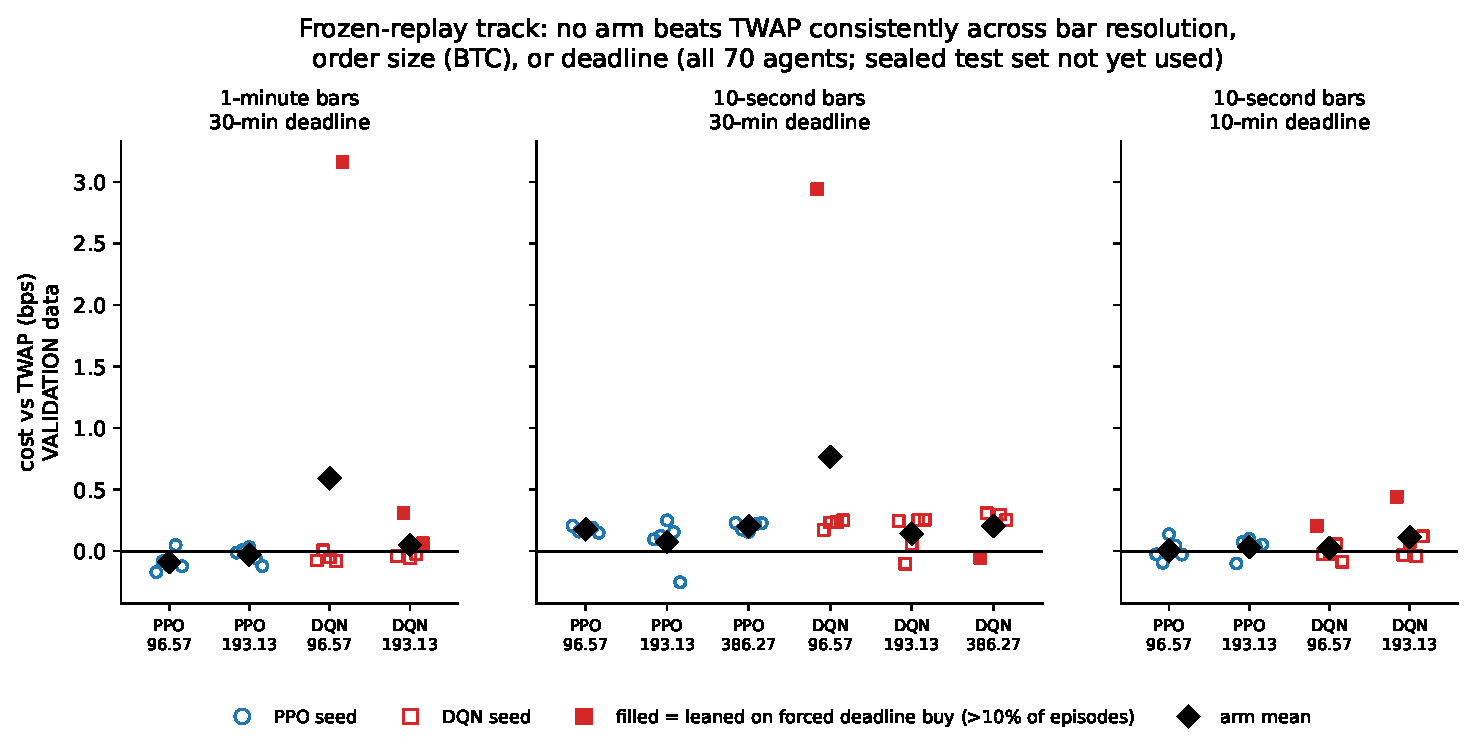
\includegraphics[width=0.95\textwidth]{l1_three_lever_null.pdf}\end{center}
\begin{itemize}
\item All 70 agents across bar resolution (1-minute, 10-second), order size (0.5\%, 1\%,
2\% of daily volume) and deadline (30, 10 minutes).
\item No arm beats TWAP consistently; on 10-second bars at 30 minutes the agents are
consistently worse.
\item The best-looking arm (PPO, 96.57 BTC, 1-minute bars: $-0.089$, 4/5 cheaper) is within
chance expectation for 14 screened arms and receives no special treatment: every arm sits
the same one-shot sealed exam.
\item Six DQN runs show the same deadline-leaning failure as the reactive track (filled markers).
\item Integrity notes: four legacy stub runs were exposed by a census, retracted and
retrained (the arm's true figure is three times weaker than the stub-based one); fill-in
comparability was proven by a bit-exact sibling retrain.
\end{itemize}

\subsection*{Frozen-replay arm summary (table)}
\begin{center}\resizebox{0.8\textwidth}{!}{% Auto-generated from the 70 L2 agents' meta.json files (VALIDATION data).
\begin{tabular}{llrrrr}
\toprule
panel & arm & pooled vs TWAP & cheaper & flagged & across-seed \\
 & & (bps) & seeds & seeds & $p$ \\
\midrule
1-min bars, 30-min & PPO 96.57 & -0.0890 & 4/5 & 0/5 & 0.037 \\
1-min bars, 30-min & PPO 193.13 & -0.0297 & 3/5 & 0/5 & 0.167 \\
1-min bars, 30-min & DQN 96.57 & +0.5920 & 3/5 & 1/5 & 0.796 \\
1-min bars, 30-min & DQN 193.13 & +0.0505 & 3/5 & 2/5 & 0.750 \\
\midrule
10-s bars, 30-min & PPO 96.57 & +0.1779 & 0/5 & 0/5 & 1.000 \\
10-s bars, 30-min & PPO 193.13 & +0.0740 & 1/5 & 0/5 & 0.781 \\
10-s bars, 30-min & PPO 386.27 & +0.2010 & 0/5 & 0/5 & 1.000 \\
10-s bars, 30-min & DQN 96.57 & +0.7663 & 0/5 & 1/5 & 0.884 \\
10-s bars, 30-min & DQN 193.13 & +0.1417 & 1/5 & 0/5 & 0.940 \\
10-s bars, 30-min & DQN 386.27 & +0.2049 & 1/5 & 1/5 & 0.981 \\
\midrule
10-s bars, 10-min & PPO 96.57 & +0.0066 & 3/5 & 0/5 & 0.562 \\
10-s bars, 10-min & PPO 193.13 & +0.0324 & 1/5 & 0/5 & 0.797 \\
10-s bars, 10-min & DQN 96.57 & +0.0244 & 3/5 & 1/5 & 0.672 \\
10-s bars, 10-min & DQN 193.13 & +0.1133 & 2/5 & 1/5 & 0.867 \\
\bottomrule
\end{tabular}}\end{center}
\begin{itemize}
\item Pooled result, seeds cheaper, flagged seeds and consistency for all 14 arms.
\item Validation data by design; test columns are added by the sealed exam.
\end{itemize}

\subsection*{The size lever}
\begin{center}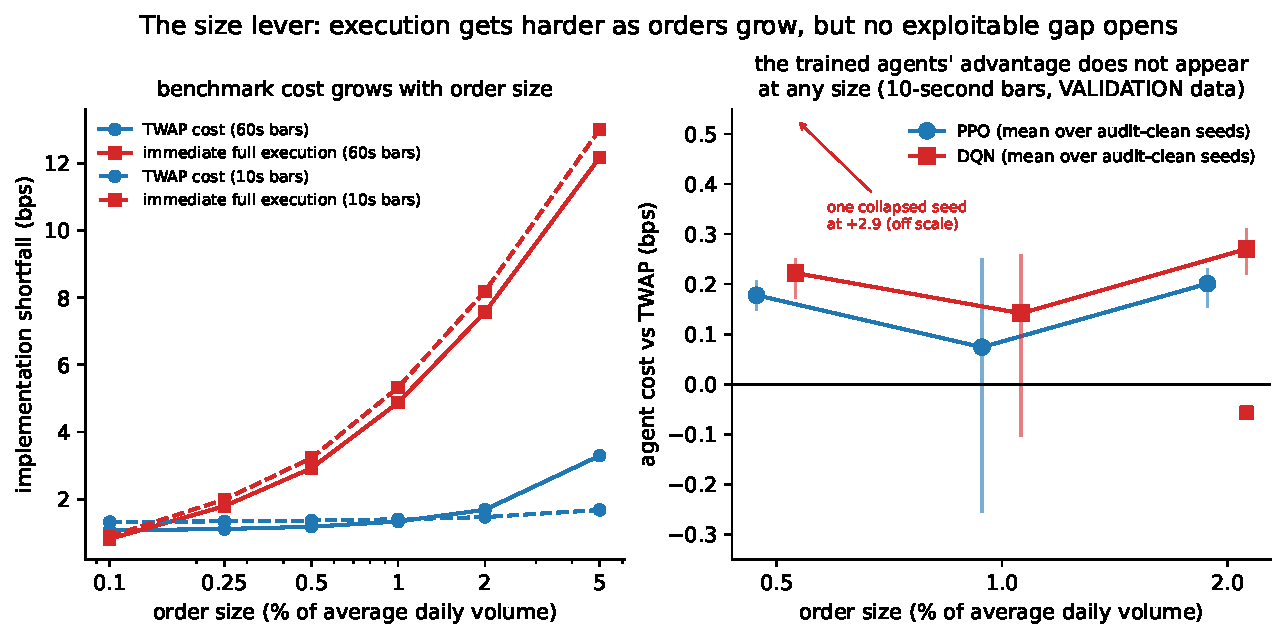
\includegraphics[width=0.95\textwidth]{l2_size_sweep.pdf}\end{center}
\begin{itemize}
\item Benchmark execution cost grows steeply with order size (to ${\sim}13$\,bps at $5\%$
of daily volume): the execution problem gets genuinely harder.
\item No exploitable agent advantage opens at any trained size; one collapsed DQN seed is
marked off scale.
\end{itemize}

\clearpage
\subsection*{Frozen-replay per-run detail (appendix table)}
\begin{itemize}
\item Every one of the 70 agents: validation result and deadline-leaning share. The table
flows over the following pages.
\item DL marks the forced deadline purchase completing more than $10\%$ of episodes.
\end{itemize}
\begin{center}\scriptsize% Auto-generated: all 70 L2 agents, per seed (VALIDATION data; test columns follow
% the sealed exam). resid = share of episodes finished by the forced deadline buy.
% LONGTABLE: flows across pages; include directly (no float, no resizebox).
\begin{longtable}{llrrr}
\toprule
panel & arm & seed & vs TWAP (bps) & resid \\
\midrule
\endhead
1-min bars, 30-min & PPO 96.57 & 0 & -0.1707 & 0.8\% \\
1-min bars, 30-min & PPO 96.57 & 1 & -0.0834 & 0.2\% \\
1-min bars, 30-min & PPO 96.57 & 2 & -0.1169 & 0.5\% \\
1-min bars, 30-min & PPO 96.57 & 3 & +0.0487 & 1.0\% \\
1-min bars, 30-min & PPO 96.57 & 4 & -0.1230 & 0.5\% \\
1-min bars, 30-min & PPO 193.13 & 0 & -0.0118 & 2.0\% \\
1-min bars, 30-min & PPO 193.13 & 1 & +0.0094 & 0.2\% \\
1-min bars, 30-min & PPO 193.13 & 2 & +0.0314 & 1.8\% \\
1-min bars, 30-min & PPO 193.13 & 3 & -0.0562 & 1.2\% \\
1-min bars, 30-min & PPO 193.13 & 4 & -0.1214 & 0.8\% \\
1-min bars, 30-min & DQN 96.57 & 0 & -0.0764 & 0.0\% \\
1-min bars, 30-min & DQN 96.57 & 1 & +0.0060 & 0.5\% \\
1-min bars, 30-min & DQN 96.57 & 2 & -0.0512 & 0.8\% \\
1-min bars, 30-min & DQN 96.57 & 3 & -0.0793 & 0.0\% \\
1-min bars, 30-min & DQN 96.57 & 4 & +3.1610 & 97.8\% \textbf{DL} \\
1-min bars, 30-min & DQN 193.13 & 0 & -0.0433 & 1.5\% \\
1-min bars, 30-min & DQN 193.13 & 1 & +0.3100 & 36.8\% \textbf{DL} \\
1-min bars, 30-min & DQN 193.13 & 2 & -0.0553 & 0.2\% \\
1-min bars, 30-min & DQN 193.13 & 3 & -0.0224 & 1.5\% \\
1-min bars, 30-min & DQN 193.13 & 4 & +0.0632 & 11.8\% \textbf{DL} \\
\midrule
10-s bars, 30-min & PPO 96.57 & 0 & +0.2056 & 0.0\% \\
10-s bars, 30-min & PPO 96.57 & 1 & +0.1587 & 0.0\% \\
10-s bars, 30-min & PPO 96.57 & 2 & +0.1846 & 0.2\% \\
10-s bars, 30-min & PPO 96.57 & 3 & +0.1919 & 0.0\% \\
10-s bars, 30-min & PPO 96.57 & 4 & +0.1488 & 0.2\% \\
10-s bars, 30-min & PPO 193.13 & 0 & +0.0956 & 0.2\% \\
10-s bars, 30-min & PPO 193.13 & 1 & +0.1229 & 0.2\% \\
10-s bars, 30-min & PPO 193.13 & 2 & +0.2496 & 0.0\% \\
10-s bars, 30-min & PPO 193.13 & 3 & +0.1552 & 0.5\% \\
10-s bars, 30-min & PPO 193.13 & 4 & -0.2533 & 5.5\% \\
10-s bars, 30-min & PPO 386.27 & 0 & +0.2294 & 0.2\% \\
10-s bars, 30-min & PPO 386.27 & 1 & +0.1743 & 0.0\% \\
10-s bars, 30-min & PPO 386.27 & 2 & +0.1565 & 0.0\% \\
10-s bars, 30-min & PPO 386.27 & 3 & +0.2174 & 0.0\% \\
10-s bars, 30-min & PPO 386.27 & 4 & +0.2272 & 0.0\% \\
10-s bars, 30-min & DQN 96.57 & 0 & +2.9426 & 97.8\% \textbf{DL} \\
10-s bars, 30-min & DQN 96.57 & 1 & +0.1728 & 7.8\% \\
10-s bars, 30-min & DQN 96.57 & 2 & +0.2327 & 0.0\% \\
10-s bars, 30-min & DQN 96.57 & 3 & +0.2341 & 0.5\% \\
10-s bars, 30-min & DQN 96.57 & 4 & +0.2493 & 0.0\% \\
10-s bars, 30-min & DQN 193.13 & 0 & +0.2441 & 0.0\% \\
10-s bars, 30-min & DQN 193.13 & 1 & -0.1025 & 10.0\% \\
10-s bars, 30-min & DQN 193.13 & 2 & +0.0570 & 0.5\% \\
10-s bars, 30-min & DQN 193.13 & 3 & +0.2537 & 0.2\% \\
10-s bars, 30-min & DQN 193.13 & 4 & +0.2561 & 0.5\% \\
10-s bars, 30-min & DQN 386.27 & 0 & -0.0569 & 27.0\% \textbf{DL} \\
10-s bars, 30-min & DQN 386.27 & 1 & +0.3082 & 1.0\% \\
10-s bars, 30-min & DQN 386.27 & 2 & +0.2214 & 1.0\% \\
10-s bars, 30-min & DQN 386.27 & 3 & +0.2978 & 0.0\% \\
10-s bars, 30-min & DQN 386.27 & 4 & +0.2537 & 0.0\% \\
\midrule
10-s bars, 10-min & PPO 96.57 & 0 & -0.0262 & 0.2\% \\
10-s bars, 10-min & PPO 96.57 & 1 & -0.0946 & 0.2\% \\
10-s bars, 10-min & PPO 96.57 & 2 & +0.1367 & 0.0\% \\
10-s bars, 10-min & PPO 96.57 & 3 & +0.0450 & 0.0\% \\
10-s bars, 10-min & PPO 96.57 & 4 & -0.0280 & 0.5\% \\
10-s bars, 10-min & PPO 193.13 & 0 & -0.1008 & 1.0\% \\
10-s bars, 10-min & PPO 193.13 & 1 & +0.0741 & 1.0\% \\
10-s bars, 10-min & PPO 193.13 & 2 & +0.0985 & 1.5\% \\
10-s bars, 10-min & PPO 193.13 & 3 & +0.0373 & 1.5\% \\
10-s bars, 10-min & PPO 193.13 & 4 & +0.0529 & 0.5\% \\
10-s bars, 10-min & DQN 96.57 & 0 & +0.2065 & 26.2\% \textbf{DL} \\
10-s bars, 10-min & DQN 96.57 & 1 & -0.0264 & 0.0\% \\
10-s bars, 10-min & DQN 96.57 & 2 & -0.0275 & 0.0\% \\
10-s bars, 10-min & DQN 96.57 & 3 & +0.0553 & 0.2\% \\
10-s bars, 10-min & DQN 96.57 & 4 & -0.0861 & 1.8\% \\
10-s bars, 10-min & DQN 193.13 & 0 & +0.4411 & 48.8\% \textbf{DL} \\
10-s bars, 10-min & DQN 193.13 & 1 & -0.0312 & 3.0\% \\
10-s bars, 10-min & DQN 193.13 & 2 & +0.0772 & 0.0\% \\
10-s bars, 10-min & DQN 193.13 & 3 & -0.0401 & 0.0\% \\
10-s bars, 10-min & DQN 193.13 & 4 & +0.1193 & 0.0\% \\
\bottomrule
\end{longtable}\end{center}
\clearpage

\section*{6. Committed next steps}
\begin{itemize}
\item Frozen-replay sealed exam: the evaluator must first reproduce known validation numbers
exactly; then one shot over all 70 agents, all arms reported, multiplicity stated; gated.
\item Measured-signal extension: measure the order-flow to future-return relationship from
the L4 data and inject exactly that into the reactive simulator; the one experiment that can
change the headline; pre-registered before running.
\item Liquidity and volume profiles (feeds a VWAP benchmark); Almgren-Chriss and VWAP added
to the benchmark set; attribution (research question 3) after the extension verdict;
decision-frequency check (12 runs at 0.5\,s and 2\,s).
\end{itemize}

\section*{7. Provenance (source of truth for every number)}
\begin{center}\small
\begin{tabular}{ll}
\toprule
result & source of truth \\
\midrule
Primary campaign & \texttt{oxford\_l4/step5\_v3/} \\
Tuning + selection & \texttt{oxford\_l4/step5\_selection\_v3/} \\
Sealed confirmations & \texttt{oxford\_l4/step5\_confirm\_\{v3a,v1b\}/} \\
Sweeps + grid & \texttt{oxford\_l4/step5\_sweep\_*, step5\_grid\_*/} \\
Replication ladder & \texttt{oxford\_l4/step5\_esc\_*, step5\_xblock\_*/} \\
DQN probe + d3 & \texttt{oxford\_l4/step5\_dqnprobe\_*, step5\_d3\_*/} \\
Q-value diagnostic & \texttt{reports/diagnostics/dqn\_q\_flatness.json} \\
Per-episode distributions & \texttt{oxford\_l4/per\_episode\_v3/} \\
Environment gates & \texttt{oxford\_l4/step4\_gates\_v3.json, step3g/fairness\_*.json} \\
Frozen-replay agents & \texttt{runs/, runs\_10s/, runs\_10s\_10min/ meta.json} \\
Frozen-replay benchmark sweep & \texttt{size\_sweep\_results.json} \\
\bottomrule
\end{tabular}
\end{center}
\begin{itemize}
\item Every number in this document is generated by script from these archived files;
nothing is transcribed by hand.
\item Markdown summaries in the project documentation are convenience copies; these
artifacts are authoritative.
\end{itemize}

\end{document}
